\newcommand{\ClassPath}{../VIU_TFM_LaTeX_template}
\documentclass{\ClassPath/viu-tfm-template}
\usepackage{multicol}

\definecolor{maincolor}{HTML}{f25416}

%--------------------------------------------------------------------------
% Definiciones necesarias Modifica con tus datos
%--------------------------------------------------------------------------
\def\nombre{Gómez Olivencia, Rubén}
\def\dni{78910013-A}
\def\titulo{Aplicaciones de gestión de proyectos:\linebreak\linebreak Diagrama de Gantt}
\def\titulacion{Máster Universitario en Desarrollo de Aplicaciones y Servicios Web}
\def\curso{2022-2023}

%Los siguientes son opcionales: si no se ponen, la portada cambia un poco. Ideal para escribir artículos/trabajos cortos
\def\dirige{}
\def\convocatoria{}
\def\asignatura{Gestión de proyectos en entornos ágiles}


% importar fichero de Bibliografía
%\addbibresource{Actividad_1.bib}

\begin{document}
    \graphicspath{{../VIU_TFM_LaTeX_template/}}

    \coverpage

    \tableofcontents

\chapter{Introducción}

A la hora de gestionar proyectos hoy en día se hace uso de las denominadas metodologías ágiles. Es cierto que estas nuevas metodologías han aportado flexibilidad y mejoras, pero eso no quita para que metodologías previas (denominadas predictivas) como los \href{https://es.wikipedia.org/wiki/Diagrama_de_Gantt}{diagramas de Gantt} puedan seguir aportando gran valor en etapas iniciales de la gestión de proyectos.

Es por eso que a lo largo de este documento se van a analizar distintos programas que nos van a permitir la gestión inicial de un proyecto haciendo uso del diagrama de Gantt.


\chapter{Software de gestión: Diagramas de Gantt}
A la hora de gestionar un proyecto haciendo uso de los diagramas de Gantt hay que decidir qué \textit{software} se va a utilizar para llevar a cabo la planificación.

Este software nos debe permitir gestionar un equipo, crear las distintas etapas por las que el proyecto va a pasar, crear dependencias de tareas... Es importante realizar una buena elección, que se ajuste a las necesidades que vamos a necesitar, para que no suponga una carga o un gasto de tiempo el utilizarlo.

Es por ello que se va a realizar un análisis de distintos programas, en los que se expondrán las posibles ventajas de cada uno de ellos y para finalizar se expondrá por cuál de ellos nos hemos decantado.

A la hora de realizar el análisis y la elección se han tenido en cuenta los siguientes aspectos:
\begin{itemize}
    \item Mejor que sea \textbf{Software Libre}. Debido a las ventajas del Software Libre, nos permitirá realizar modificaciones en caso de que sea necesario para poder adaptarlo a las necesidades propias en caso de que falte alguna característica.

    \item Que sea un proyecto que \textbf{se mantenga “vivo”}. Teniendo en cuenta el punto anterior, ya sea para poder realizar una modificación propia o pedirle al desarrollador la posibilidad de implementarla, es necesario que el software se siga manteniendo y desarrollando. Aparte, eso también significará que su uso está extendido.
    \item Que sea \textbf{multiplataforma}, \textbf{o desarrollado en entorno web}. Debido a que en el equipo se hace uso de distintos sistemas operativos, es conveniente que el programa elegido se pueda utilizar en distintos sistemas operativos.

    En caso de que sea un desarrollo web, evitaríamos ese problema, pero sería interesante que tuviese sistema de control de usuarios. También es recomendable poder contar con la posibilidad de tener el sistema en nuestros propios servidores.

    \item Uso de \textbf{estándares abiertos}, sobre todo a la hora de exportar el diagrama. Suele ser lo habitual con el Software Libre, pero es recomendable saber que lo realizado se puede exportar en un formato libre que posteriormente pueda ser abierto con otro programa, por si en el futuro se decide cambiar de programa.
\end{itemize}

Teniendo en cuenta estas características, nos aseguraremos que el software elegido no nos limita durante la gestión del proyecto, y que en caso de que así sea, se pueda cambiar rápidamente por una alternativa mejor.


\section{Análisis de software}

A continuación se va a realizar el análisis de distintas aplicaciones identificando algunas de sus características, ya sean ventajas o inconvenientes, para realizar una pequeña comparativa final.

En la \href{https://en.wikipedia.org/wiki/Comparison_of_project_management_software}{Wikipedia} existe una página de software de gestión de proyectos, que nos puede servir como una guía de inicio para empezar a buscar.

\subsection{Gantt Project}

\href{https://www.ganttproject.biz/}{Gantt Project} es una aplicación de escritorio multiplataforma que tiene una larga trayectoria a sus espaldas. Es Software Libre y está escrito en Java.

Entre las ventajas que se pueden destacar es que se pueden generar reportes en formato PDF y HTML, se puede importar y exportar a/desde Microsoft Project, tiene gestión de vacaciones y es Software Libre.


\begin{center}
    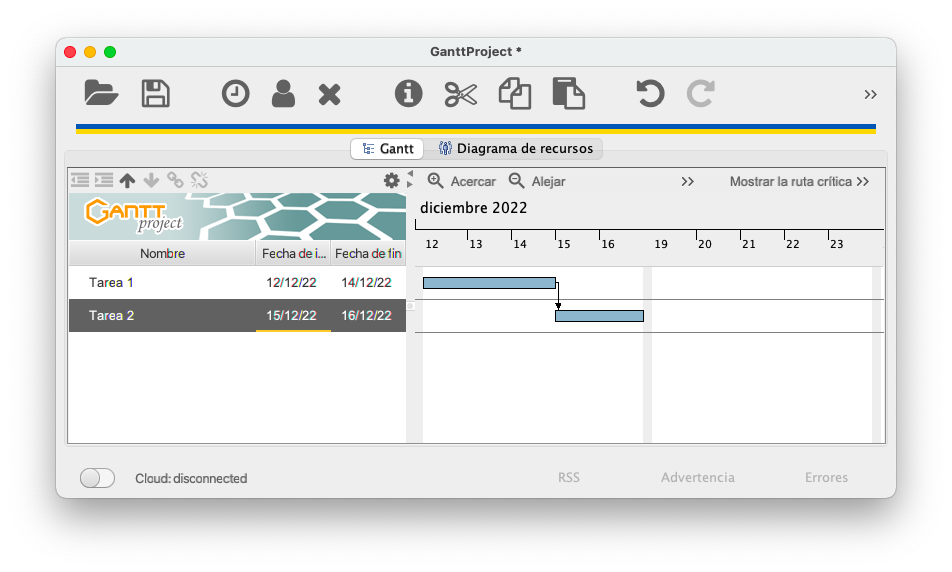
\includegraphics[width=0.7\linewidth]{img/ganttproject.png}
\end{center}

Como inconveniente se le puede poner que es una aplicación de escritorio, aunque tienen una opción de pago llamada “GanttProject Cloud” para modo colaborativo.

\subsection{Gnome Planner}
\href{https://wiki.gnome.org/Apps/Planner}{Gnome Planner} es otra aplicación de escritorio dentro del ecosistema del escritorio \href{https://www.gnome.org/}{Gnome}, muy conocido en el mundo GNU/Linux.

Esta aplicación a nivel visual, aunque es subjetivo, se puede decir que está más cuidada, y en caso de utilizar un escritorio Gnome, se integra perfectamente en lo que ya conocemos.

\begin{center}
    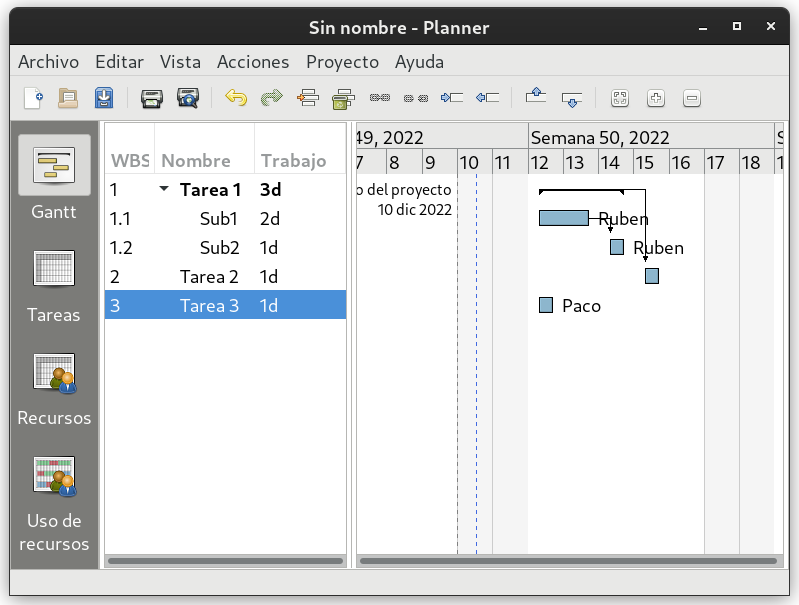
\includegraphics[width=0.7\linewidth]{img/planner.png}
\end{center}

Por otro lado, cuenta con la posibilidad de crear grupos de personas/recursos, y de manera sencilla se puede ver el listado de tareas completas y el estado de cada recurso, en qué está ocupado en el momento actual o si por el contrario está libre.

Al igual que sucede con la anterior aplicación, al ser una aplicación de escritorio limita el uso de distintos usuarios al mismo fichero/proyecto.


\subsection{Instagantt}
\href{https://instagantt.com/}{Instagantt} es una aplicación web para poder crear diagramas de Gantt que está enfocado para el gestor de proyectos \href{https://asana.com/es}{Asana}.


\begin{center}
    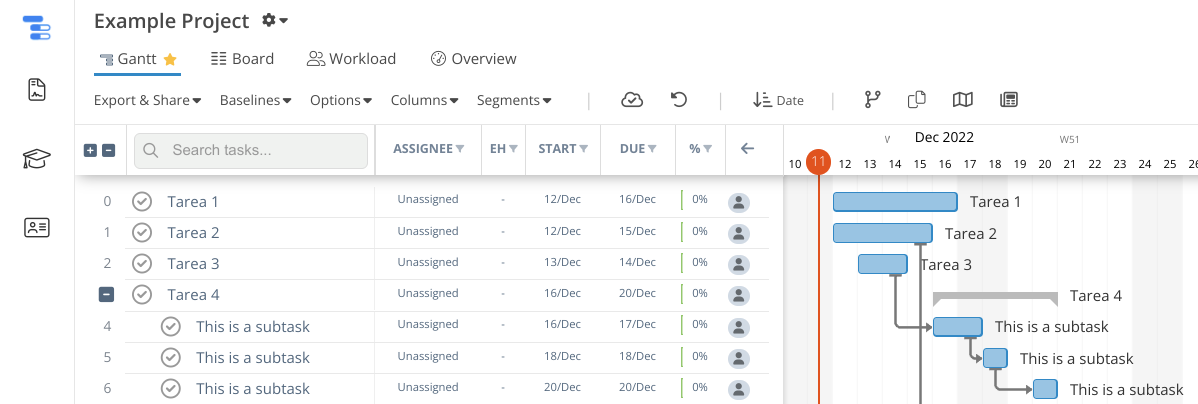
\includegraphics[frame,width=0.8\linewidth]{img/instagantt.png}
\end{center}

Instagantt tiene un periodo de prueba de 7 días, en los que se podrá hacer uso de él, pero después tiene un pago de suscripción de 7 dólares al mes para un único usuario, o 5 dólares por usuario/mes si queremos que se pueda utilizar de manera cooperativa.


\subsection{Redmine}

\href{https://www.redmine.org/}{Redmine} es un gestor de proyectos completo basado en web. Es Software Libre, está escrito en Ruby on Rails y es fácil de crear una instancia a través de contenedores Docker.

Al ser un gestor de proyectos completo tiene sus ventajas a la hora de utilizarlo dentro de una empresa, ya que desde una aplicación podemos crear incidencias, gestionar código fuente, referenciar modificaciones de código asociado a incidencias... Es una herramienta muy potente que para tener un histórico de todo lo realizado por los trabajadores y la empresa viene muy bien.

Por otro lado, su implantación no es sencilla ni rápida, ya que hay que dar de alta a los usuarios, crear distintos estados de las incidencias, crear flujos de trabajo, crear perfiles de usuarios sobre proyectos, asignarlos a usuarios...

\begin{center}
    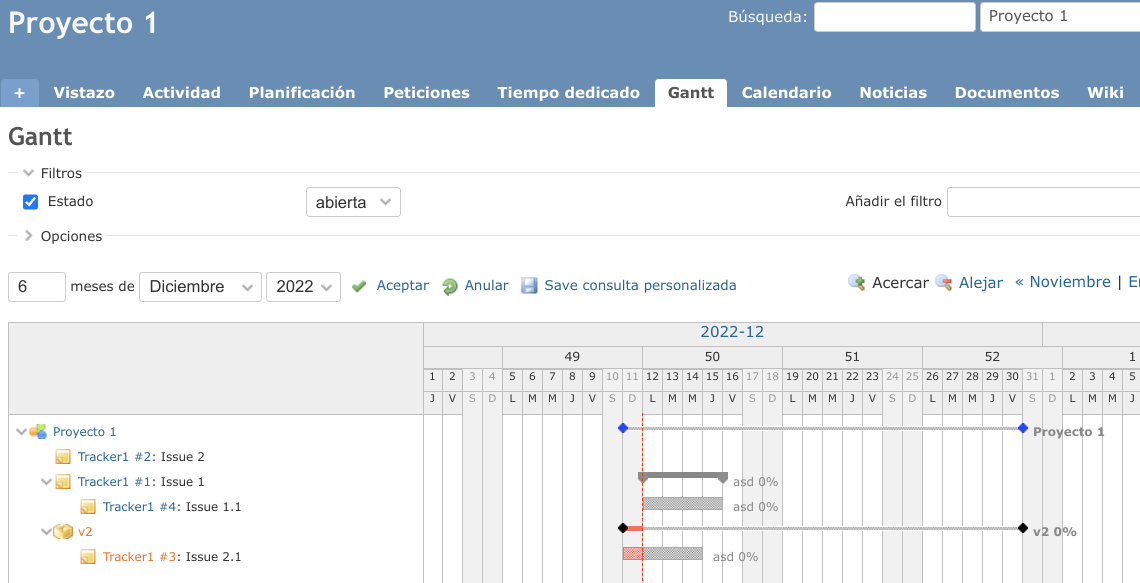
\includegraphics[frame,width=0.7\linewidth]{img/redmine.png}
\end{center}

Una vez superado lo mencionado anteriormente, como tendremos que haber ido creando las incidencias y asignarlas a los usuarios, la ventaja es que no sólo tendremos el diagrama de Gantt hecho, si no toda la gestión del proyecto, incidencias, asignaciones... Ya que todo se encuentra en la misma aplicación web.


\subsection{OpenProject}

Al igual que el caso anterior, \href{https://www.openproject.org/}{OpenProject} es un software web para la gestión de proyectos completos. También es Software Libre, también programado en Ruby on Rails, pero esta vez con la parte \textit{frontend} hecha en Angular.

Este software está pensado para el uso por parte de todos los integrantes de una empresa, para la creación de tareas, seguimiento... y levantar una instancia con Docker, una vez más,  resulta muy sencillo.

\begin{center}
    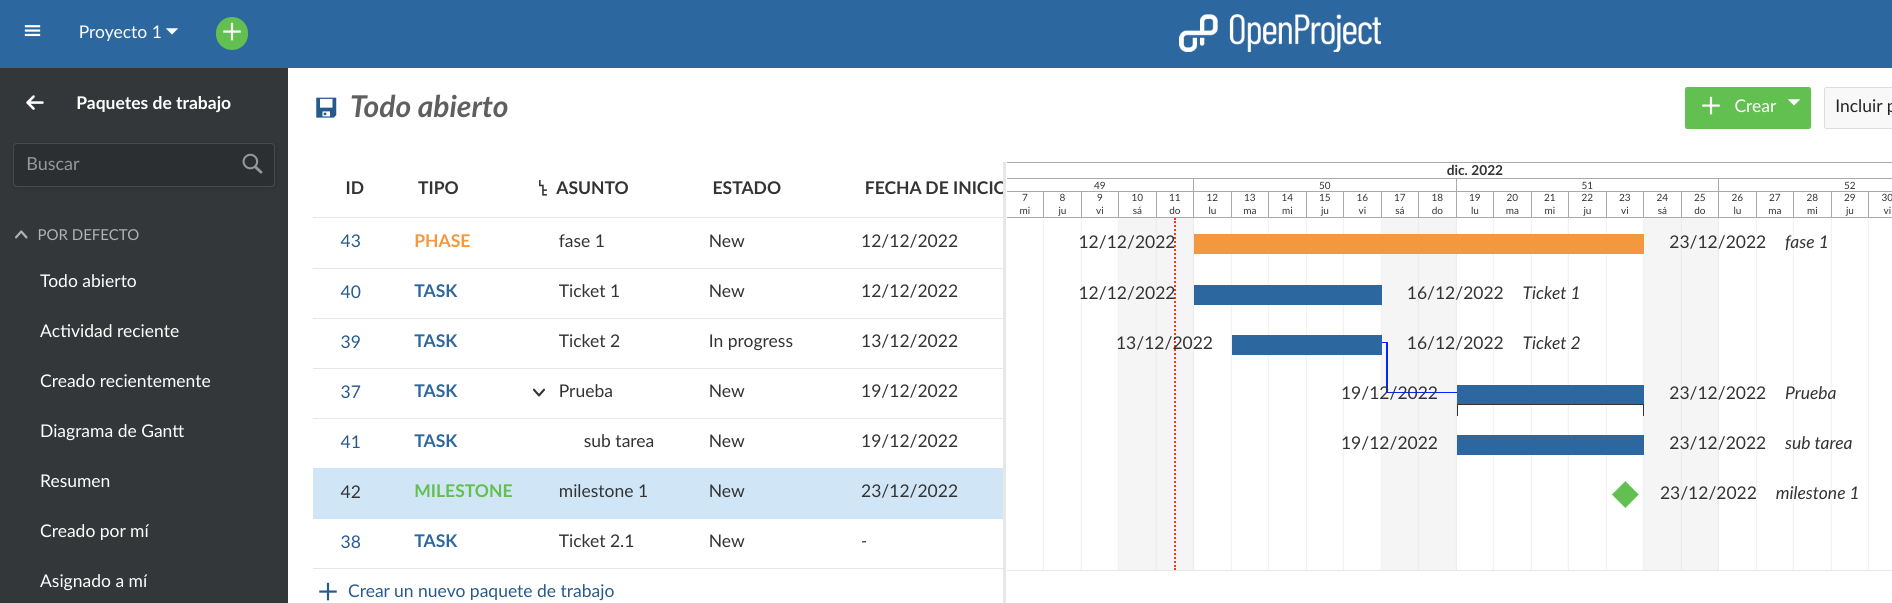
\includegraphics[frame,width=0.9\linewidth]{img/openproject.png}
\end{center}

Tal como sucedía con Redmine, hay que dar de alta a los usuarios, pero a la hora de crear las tareas, asignarlas, cambiar el estado de las mismas... es mucho más intuitivo. Ya existen estados pre-definidos, el relacionar tareas entre sí es mucho más sencillo, se pueden modificar fechas en el propio diagrama de Gantt, el aspecto visual está mucho más cuidado...

Tiene una versión “Enterprise” que cuenta con distintos añadidos, pero la versión libre es completamente funcional. El problema principal de esta aplicación es que abarca demasiado si sólo queremos crear un diagrama de Gantt.


\section{Comparativa}

A continuación, una pequeña tabla comparativa de las distintas aplicaciones analizadas:

\begin{yukitblrcol}{XXXXXX}
    & Gantt Project & Gnome Planner & Redmine & Open Project & Instagantt \\
    Software Libre & \checkmark & \checkmark & \checkmark & \checkmark & \times \\
    Multi usuario & Equipos de 2 gratis & \times & \checkmark & \checkmark & Pagando \\
    Multi plataforma & \checkmark & Linux / Windows & \checkmark & \checkmark & \checkmark \\
    Facilidad de uso & Fácil & Fácil & Complejo & Medio & Fácil \\
\end{yukitblrcol}


\section{Elección del software a utilizar}
Teniendo en cuenta que se ha analizando software muy diverso ()unos que sólo permiten la creación de diagramas de Gantt y otros que son gestores de proyecto completos, con soporte de creación de incidencias, gestión de tiempo, usuarios...) hay que tener en cuenta las necesidades actuales, para “no matar moscas a cañonazos”.

Si necesitásemos la gestión completa de un proyecto, para tener control total de tiempos por empleados, creación de incidencias, gestión de las mismas, aparte de la creación del diagrama de Gantt, la mejor opción sería Open Project.

En cambio, las necesidades actuales lo único que abarcan es la creación de un diagrama de Gantt, por lo que las funcionalidades que nos ofrece \textbf{Gantt Project} se ajustan perfectamenet.


\chapter{Creación del proyecto}

\chapter{Planteamiento}

\section{Elección de los roles}

\section{Tareas a realizar}

\section{Diagrama final}



\chapter{Conclusiones}

Aunque el p

\end{document}
